\documentclass[a4paper, 12pt]{article}
\usepackage[utf8]{inputenc}
\usepackage[T1]{fontenc}
\usepackage{times}
\usepackage[spanish]{babel}
% \usepackage{hyperref} % Paquete para hipervínculos
\usepackage[left=2.5cm, right=2.5cm, top=2.5cm, bottom=2.5cm]{geometry}
\linespread{1.5}
\usepackage{graphicx} % Required for inserting images
\usepackage{amsmath}
\usepackage{titlesec} % Paquete para el formato de los títulos

\setlength{\parindent}{0pt}

% Reducir el espacio entre los apartados del índice
\makeatletter
\renewcommand*\l@section{\@dottedtocline{1}{0em}{1.5em}}
\renewcommand*\l@subsection{\@dottedtocline{2}{1.5em}{2.5em}}
\renewcommand*\l@subsubsection{\@dottedtocline{3}{4.0em}{3.5em}}
\makeatother

\begin{document}
%-------------------------------------------------------
% PORTADA
%-------------------------------------------------------
\begin{titlepage}
	\begin{center}
		
\includegraphics[scale=0.9]{images.png}
		\vspace{1.75cm}
		
		\large
		\textbf{ESCUELA TÉCNICA SUPERIOR DE INGENIERÍA INFORMÁTICA}
		\vspace{1cm}
		
		\large
		\textbf{GRADO EN INGENIERÍA INFORMÁTICA}
		
		
		
		\large
		\textbf{Curso Académico 2023/2024}
		
		\vspace{1cm}
		\large
		\textbf{Práctica 1}
		
		\vspace{2cm}
		
		\large
		\textbf{DETECCIÓN DE SEÑALES VIALES}
		
		\vspace{2cm}
		
		\large
		Cristian Fernando Calva Troya \\
		Luis Ovejero Martín \\
		Jaime Rueda Carpintero
		\vspace{1cm}
	\end{center}
\end{titlepage}

\newpage
\thispagestyle{empty} 
\mbox{} 

\newpage
%-------------------------------------------------------
% Tabla de figuras
%-------------------------------------------------------
\newpage
\listoffigures
\newpage

%-------------------------------------------------------
% Tabla de contenidos
%-------------------------------------------------------
{\small
	\tableofcontents 
}
\newpage

%-------------------------------------------------------
% 1. Introducción
%-------------------------------------------------------
\section{Introducción}
%-------------------------------------------------------
% 2. OBJETIVOS Y METODOLOGIAS
%-------------------------------------------------------
\section{Objetivos y metodología}

\subsection{Descripción del problema}

\subsection{Objetivos}
3 pag.
\subsection{Tecnologías}

%-------------------------------------------------------
% 3. DESCRIPCIÓN INFORMMATICA
%-------------------------------------------------------

\section{Creación de la aplicación}
\subsection{Normalización}
\subsubsection{Corrección de color}
\subsubsection{Corrección de ángulo}
\begin{figure}[h]
	\centering
	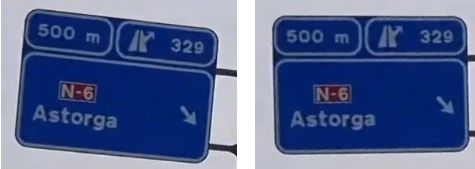
\includegraphics[width=0.8\linewidth]{img/norma_angulo}
	\caption{Corrección de angulo de la imagen}
	\label{fig:normaangulo}
\end{figure}

Otro de los problemas presentes a la hora de procesar las imagenes, para su detección, es la posición de los objetos a detectar. En ocasiones, ya sea por el ángulo de la cámara o la misma posición del cartel respeto a nosotros, puede ocurrir un cierto desfase en el angulo deseado. En la \textbf{Fig. 1} podemos observar un pequeño ejemplo del problema inicial y el resultado deseado, que nos dará una mejor detección de las secciones. Para poder abarcar el problema hemos optado por realizar una corrección a la imagen completa. 

Los pasos a seguir para conseguir el angulo de desfase son los siguientes:



\begin{quote}
	\textbf{1.} Aplicamos una detección de color azul ya que respecto a las diferentes pruebas, ha dado mejores resultados para eliminar las zonas no deseadas y poder centrarnos en las secciones más azules (los paneles deseados.) En la \textbf{Fig. x} podemos ver un ejemplo de los posibles resultados.
	\begin{figure}[h]
		\centering
		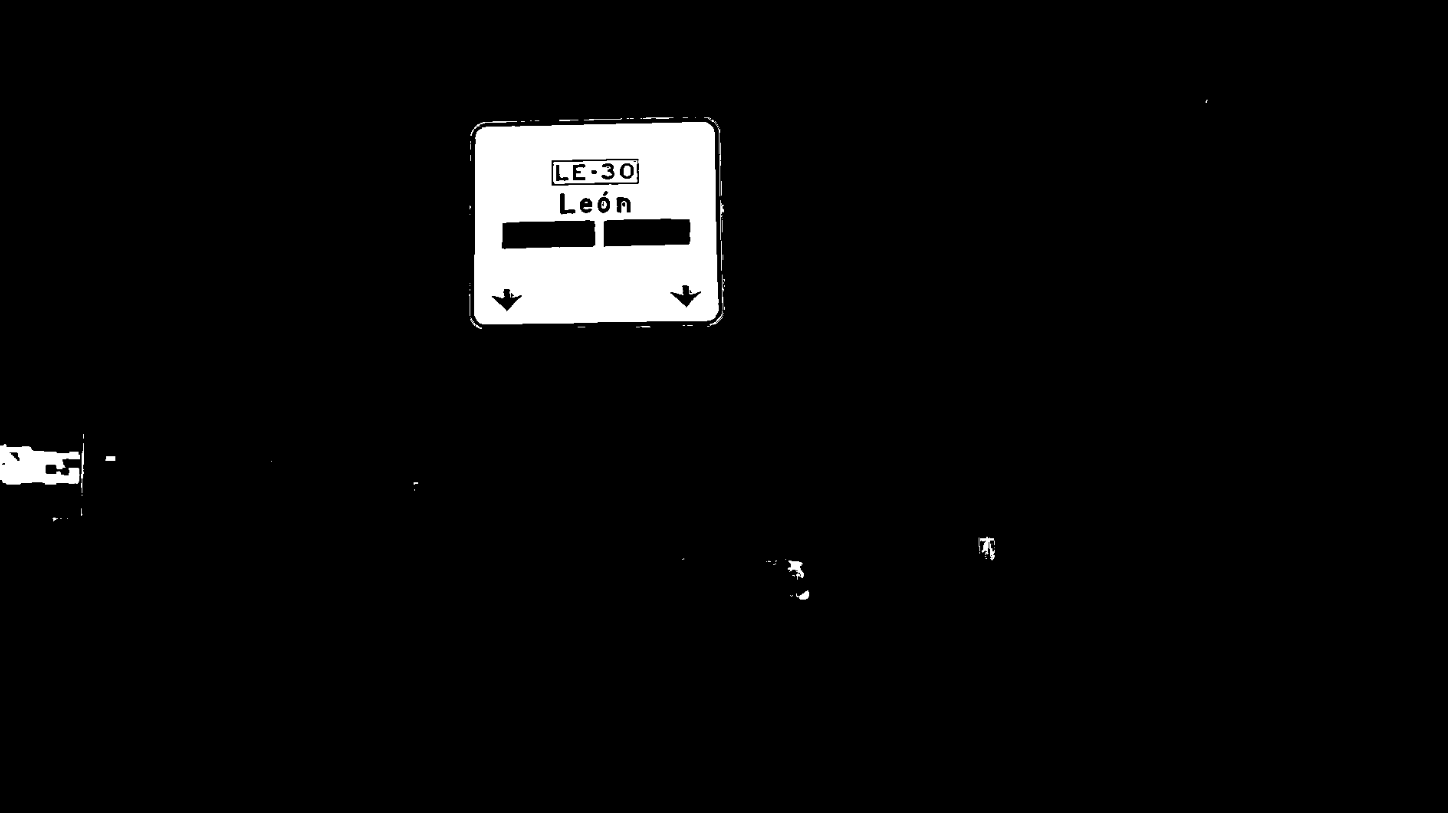
\includegraphics[width=0.6\linewidth]{img/image_blue_f}
		\caption{Imagen tras aplicar filtro azul}
		\label{fig:imagebluef}
	\end{figure}
	
	\textbf{2.} Realizamos una detección de bordes horizontales. Ya que haremos la corrección en función de como estén estos orientados. En la \textbf{Fig. x} se ve que conseguimos las secciones deseadas.
	
	\begin{figure}[h]
		\centering
		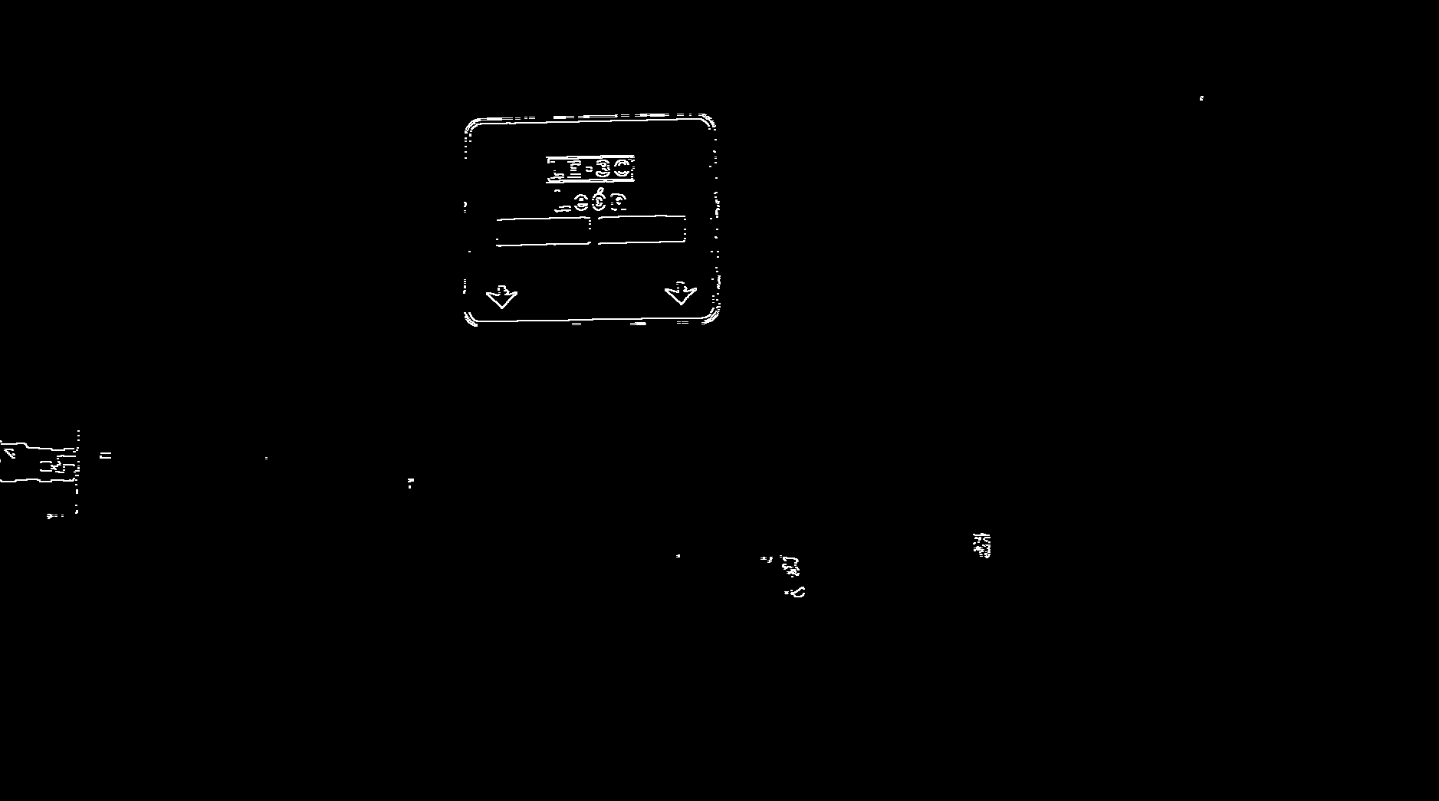
\includegraphics[width=0.6\linewidth]{img/image_boder_h}
		\caption{Imagen tras aplicar sobel}
		\label{fig:imageboderh}
	\end{figure}
	\textbf{3.} Finalmente con el algoritmo de Hough extraemos líneas presentes en la imagen, dando como resultado las rectas horizontales. En la \textbf{Fig. x} se visualizan las rectas detectadas, y se calcula el angulo de cada uno de ellas haciendo uso de las coordenadas $(x, y)$ y $(x2, y2)$, de estas nos quedaremos con un desfase intermedio. Finalmente con el ángulo de cada imagen, corregimos el giro sobre la imagen original, tal y como se muestra en la \textbf{Fig. x}.
	
	\begin{figure}[h]
		\centering
		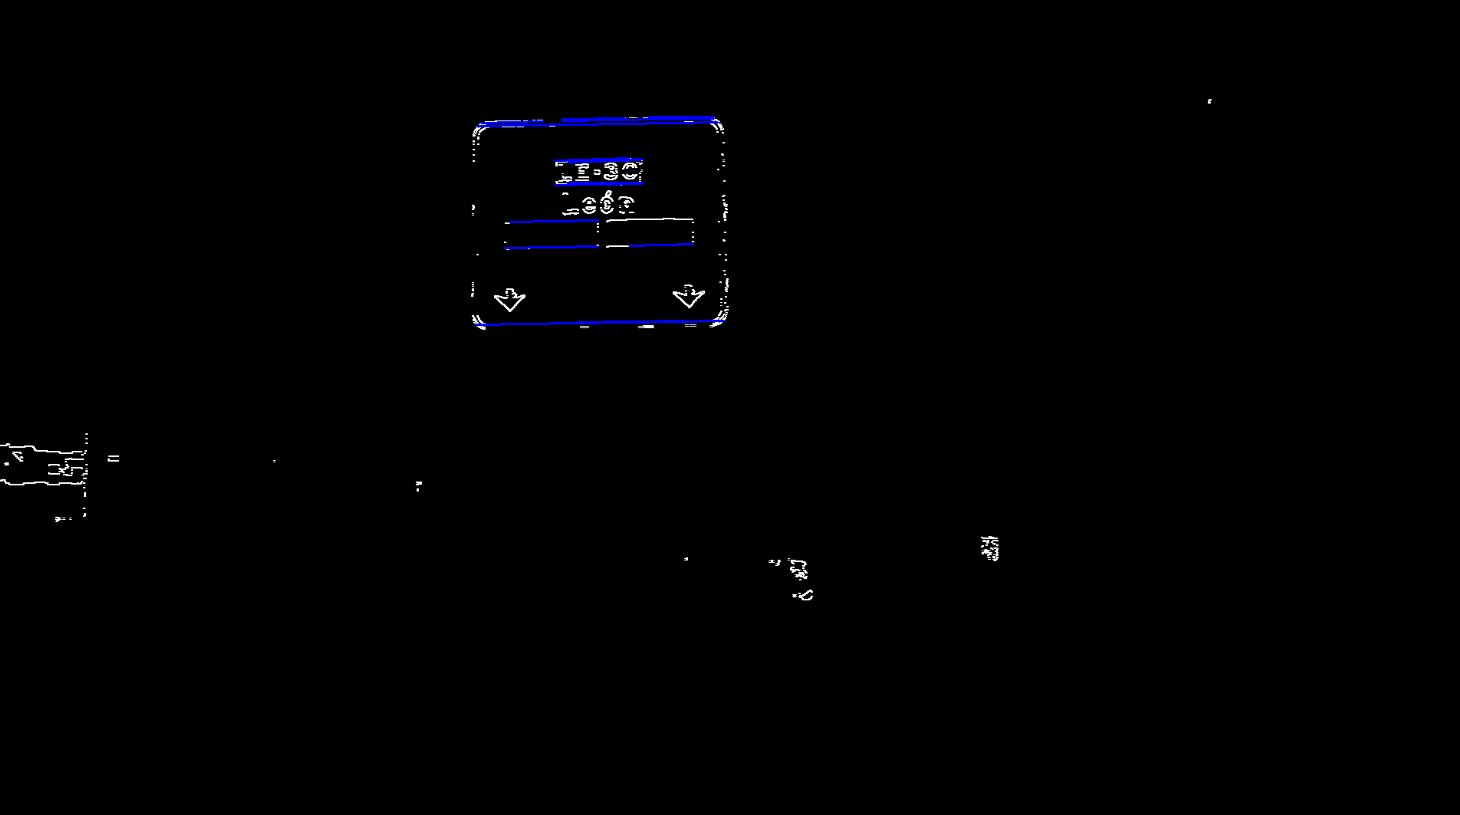
\includegraphics[width=0.6\linewidth]{img/image_with_lines+}
		\caption{Imagen tras detectar lineas y ángulos de desfase}
		\label{fig:imagewithlines}
	\end{figure}
	
	\begin{figure}[h]
		\centering
		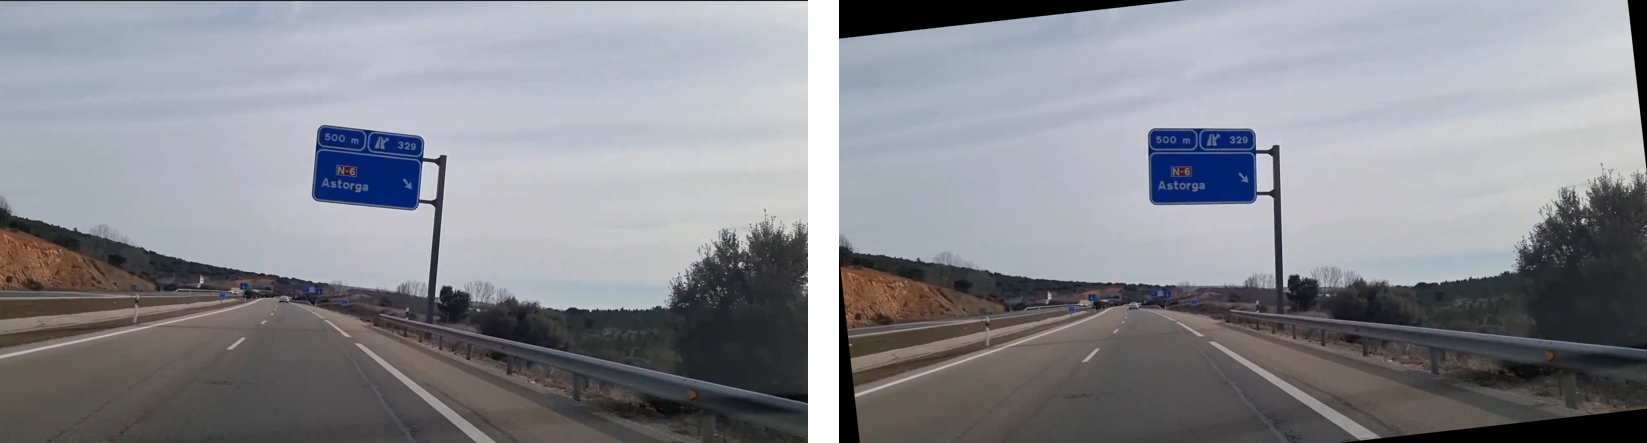
\includegraphics[width=0.7\linewidth]{img/00057_co}
		\caption{Corrección de angulo de imagen}
		\label{fig:00057co}
	\end{figure}
	
\end{quote}
\subsection{MSER}

\subsection{Correlación por máscaras}
\subsubsection{Mascara ideal}

\begin{figure}[h]
	\centering
	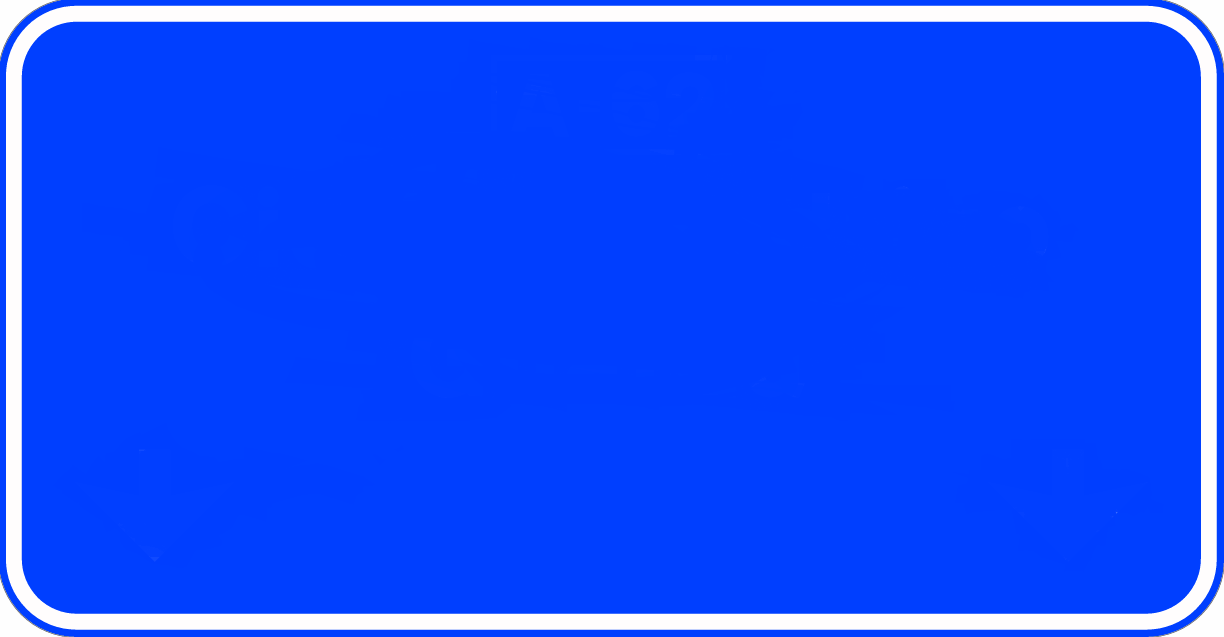
\includegraphics[width=0.4\linewidth]{img/ideal_mask}
	\caption{Panel ideal}
	\label{fig:idealmask}
\end{figure}

Para la correcta comprobación de que si una imagen ya filtrada por color es un panel deseado, necesitamos un panel de referencia, para poder indicar como debería ser un panel detectado de forma aproximada.


En la \textbf{Fig. 1} podemos ver la imagen de la que partimos para realizar esa mascara ideal que utilizaremos posteriormente. Esta imagen inicial se extrae de la Norma 8.1-IC de señalización vertical de carreteras en España \textbf{[1]}.

Para poder crear la matriz de 1's (para azules) y 0's (para no azules) hacemos uso de un filtro de color. Antes de poder hacer uso del filtro de color necesitamos cambiar el formato de la imagen de \textbf{BGR} a \textbf{HSV}. Este cambio es fundamental porque en el espacio de color HSV, el componente Hue permite una separación clara del color azul, independientemente de las variaciones de iluminación y sombra. Esta conversión y filtrado mejoran significativamente el procesamiento y permiten realizar comparaciones directas con un panel de referencia, facilitando la verificación.

\begin{figure}[h]
	\centering
	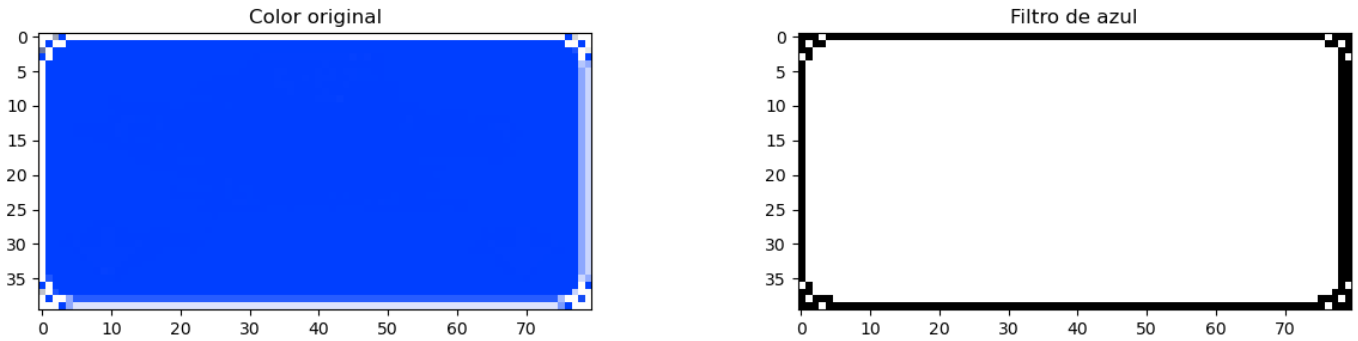
\includegraphics[width=0.9\linewidth]{img/ideal_mask_resized_and_filtered}
	\caption{Panel ideal redimensionado y filtrado por color}
	\label{fig:idealmaskresizedandfiltered}
\end{figure}

Ya que nos encontraremos con diferentes paneles de diferentes tamaños, establecemos una tamaño estandar de (80x40) a redimensionar para todos los paneles, tanto detectados como para el ideal. Tras aplicar esta redimensión podemos ya aplicar el filtro de color a nuestro panel, en la \textbf{Fig. 2} podemos ver el resultado de este proceso con el panel ideal.
\begin{figure}[h]
	\centering
	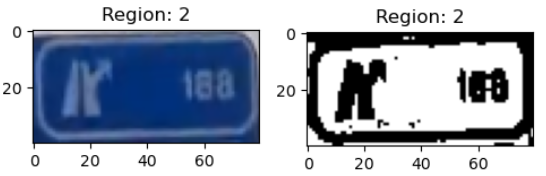
\includegraphics[width=0.7\linewidth]{img/sections}
	\caption{Panel detectado redimensionado y filtrado por color}
	\label{fig:sections}
\end{figure}

Respecto a los paneles detectados en la \textbf{Fig. 3} podemos ver un ejemplo de su proceso de redimensionado y filtrado por color. De esta manera ya podriamos realizar una comparación y correlación entre detectado/ideal.

\subsubsection{Filtrado por correlación ideal/detectado}
Llegados a este punto quedaría decidir que paneles recibidos son lo suficientemente parecidos al panel ideal. Para ellos realizamos:
\begin{quote}
	\textbf{1.} Una suma de cuantos píxeles azules tiene nuestra máscara ideal. Teniendo en cuenta que es una máscara de 0's y 1's queda bajo la siguiente operación:
	\begin{equation}
		B = \sum_{i = 0}^{39}\sum_{j = 0}^{79} I(i, j)
	\end{equation}
	
	\textbf{2.} Calcular la cantidad de azules que tiene nuestra detección. De igual forma que en el paso anterior:
	\begin{equation}
		B' = \sum_{i = 0}^{39}\sum_{j = 0}^{79} I'(i, j)
	\end{equation}
	\textbf{3.} Calcular un porcentaje de correlación normalizado entre [0,1]. Simplemente haciendo una proporción de $B'$ sobre $B$, en caso de que $B'$ supere a $B$ descartamos esta detección poniendo su proporción a 0. Quedando:
	\begin{equation}
		C = 
		\begin{cases} 
			B'/B & \text{si } B' \leq B, \\
			0 & \text{si } B \leq B'.
		\end{cases}
	\end{equation}
	
	\textbf{4.} Descartamos aquellos valores $C$ que superen un umbral. En este caso se ha puesto uno mínimo de 0'4.
\end{quote}

Posterior a estos pasos nos quedarían las secciones más fiables a la detección deseada, pero nos quedaría eliminar posibles detecciones repetidas.
\subsection{Eliminación de regiones repetidas}

\subsection{Validación}

\subsection{...}


%-------------------------------------------------------
\section{Conclusiones y trabajos futuros}
3 pag.
%-------------------------------------------------------
\section{Referencias}
[1] https://www.fomento.gob.es/az.bbmf.web/documentacion/pdf/re3723.pdf
%-------------------------------------------------------
\end{document}
